\documentclass[14pt]{beamer}
\usetheme{Dresden}
\usecolortheme{orchid}

\usepackage{xcolor}
\usepackage{listings}
\usepackage{courier}
\usepackage{graphicx}
\usepackage{amsmath}
\usepackage{algorithm2e}
\usepackage{multicol}

\usefonttheme[onlymath]{serif}

\definecolor{mGreen}{rgb}{0,0.6,0}
\definecolor{mGray}{rgb}{0.5,0.5,0.5}
\definecolor{mPurple}{rgb}{0.8,0,0.82}
\definecolor{backgroundColour}{rgb}{0.95,0.95,0.92}
\definecolor{lightBlue}{rgb}{0.1, 0.1, 0.8}

\lstdefinestyle{CStyle}{
    backgroundcolor=\color{backgroundColour},   
    commentstyle=\color{mGreen},
    keywordstyle=\color{magenta},
    numberstyle=\tiny\color{mGray},
    stringstyle=\color{mPurple},
    basicstyle=\footnotesize\ttfamily,
    breakatwhitespace=false,         
    breaklines=true,                 
    captionpos=b,                    
    keepspaces=true,                 
    numbers=left,                    
    numbersep=5pt,                  
    showspaces=false,                
    showstringspaces=false,
    showtabs=false,                  
    tabsize=2,
    language=C
}

\lstdefinestyle{Ctable}{
    backgroundcolor=\color{backgroundColour},   
    commentstyle=\color{mGreen},
    keywordstyle=\color{magenta},
    numberstyle=\tiny\color{mGray},
    stringstyle=\color{mPurple},
    basicstyle=\footnotesize\ttfamily,
    breakatwhitespace=false,         
    breaklines=true,                 
    captionpos=b,                    
    keepspaces=true,                                  
    showspaces=false,                
    showstringspaces=false,
    showtabs=false,                  
    tabsize=2,
    language=C
}

\lstdefinestyle{pseudo}{
        basicstyle=\ttfamily\footnotesize,
        keywordstyle=\color{lightBlue},
        morekeywords={BEGIN,END,IF,ELSE,ENDIF,ELSEIF,PRINT,WHILE,RETURN,ENDWHILE,DO,FOR,TO,IN,ENDFOR,BREAK,INPUT,READ},
        morecomment=[l]{//},
        commentstyle=\color{mGreen}
}

\lstset{basicstyle=\footnotesize\ttfamily,breaklines=true}
\lstset{framextopmargin=50pt,tabsize=2}

\title{ENGG1003 - Friday Week 3}
\subtitle{More Sequence Examples\\Maybe More Flow Control}
\author{Brenton Schulz}
\institute{University of Newcastle}
\date{\today}


\begin{document}
\titlepage


\begin{frame}
\frametitle{Assessment Task Rules}
\begin{center}
...Jump to rules PDF
\end{center}
\end{frame}

\begin{frame}
\frametitle{Easy(ish) Assessment Task Example}
{\small Write a C program which generates a sequence of numbers:
\begin{equation*}
x_1, x_2, x_3, ...
\end{equation*}
with the iterative equation:
\begin{equation*}
x_n = 3x_{n-1} + 2x_{n-2}
\end{equation*}
and initial conditions:
\begin{align*}
x_1 = 3,~ x_2 = 1
\end{align*}
The program should exit after printing ($x_8$ or an $x_n > 100$).
}
\end{frame}

\begin{frame}[fragile]
\frametitle{Easy(ish) Assessment Task Example}
The program's output format is:
\begin{lstlisting}[style=pseudo]
n x<newline>
\end{lstlisting}
For the values given, the output is:
\begin{lstlisting}[style=pseudo]
1 3.000000
2 1.000000
3 9.000000
4 29.000000
5 105.000000
\end{lstlisting}
\end{frame}

\begin{frame}
\frametitle{Easy(ish) Assessment Task Example}
\begin{itemize}
\item What do we need to do?
	\begin{itemize}
		\item Set up variables
		\item Give some initial values
		\item Implement the equation
		\item Print the initial values
		\item Write a \texttt{while()} loop
		\item Get the exit condition correct
		\item Print results
		\item Wrap the whole thing in \texttt{main()}
	\end{itemize}
\end{itemize}
\end{frame}

\begin{frame}[fragile]
\frametitle{Set up variables}
Question didn't specify, but lets assume \texttt{float}
\begin{lstlisting}[style=CStyle]
float xn, xnm1, xnm2;
int n; 
\end{lstlisting}
\end{frame}

\begin{frame}[fragile]
\frametitle{Give some initial values}
Question gave us:
\begin{align*}
x_1 = 3,~ x_2 = 1
\end{align*}
Be careful with \texttt{xnm1} and \texttt{xnm2}, where are we starting? 
\begin{lstlisting}[style=CStyle]
float xn, xnm1 = 1, xnm2 = 3;
int n = 3; // The first unknown is x for n=3
\end{lstlisting}
\end{frame}

\begin{frame}[fragile]
\frametitle{Implement the equation}
\begin{equation*}
x_n = 3x_{n-1} + 2x_{n-2}
\end{equation*}
\begin{lstlisting}[style=CStyle]
float xn, xnm1 = 1, xnm2 = 3;
int n = 3; // The first unknown is x for n=3

xn = 3.0*xnm1 + 2*xnm2;
\end{lstlisting}
That calculates $x_3$, but how does the program ``advance in time''?
\end{frame}

\begin{frame}[fragile]
\frametitle{Implement the equation}
Shift all the variables ``forward in time'' with:
\begin{lstlisting}[style=CStyle]
float xn, xnm1 = 1, xnm2 = 3;
int n = 3; // The first unknown is x for n=3

xn = 3.0*xnm1 + 2*xnm2;
xnm2 = xnm1;
xnm1 = xn;
\end{lstlisting}
\end{frame}

\begin{frame}[fragile]
\frametitle{Print the initial values}
\begin{lstlisting}[style=CStyle]
float xn, xnm1 = 1, xnm2 = 3;
int n = 3; // The first unknown is x for n=3

// x1 and x2 given so just hard code n
printf("1 %f\n", xnm2);
printf("2 %f\n", xnm1);

xn = 3.0*xnm1 + 2*xnm2;
xnm2 = xnm1;
xnm1 = xn;
\end{lstlisting}
\end{frame}

\begin{frame}[fragile]
\frametitle{Write a \texttt{while()} loop}
We need to calculate $x_n$ more than once, so:
\begin{lstlisting}[style=CStyle]
float xn, xnm1 = 1, xnm2 = 3;
int n = 3; // The first unknown is x for n=3

// x1 and x2 given so just hard code n
printf("1 %f\n", xnm2);
printf("2 %f\n", xnm1);

while( /* something */ ) {
	xn = 3.0*xnm1 + 2*xnm2;
	xnm2 = xnm1;
	xnm1 = xn;
}
\end{lstlisting}
\end{frame}

\begin{frame}[fragile]
\frametitle{Get the exit condition correct}
The value of n goes from 1 to 8, and xn must remain below 100:
\begin{lstlisting}[style=CStyle]
float xn, xnm1 = 1, xnm2 = 3;
int n = 3; // The first unknown is x for n=3
// x1 and x2 given so just hard code n
printf("1 %f\n", xnm2);
printf("2 %f\n", xnm1);
while( (n <= 8) && (xn < 100) ) {
	xn = 3.0*xnm1 + 2*xnm2;
	xnm2 = xnm1;
	xnm1 = xn;
	n++;
}
\end{lstlisting}
\end{frame}

\begin{frame}[fragile]
\frametitle{Print results}
\begin{lstlisting}[style=CStyle]
float xn, xnm1 = 1, xnm2 = 3;
int n = 3; // The first unknown is x for n=3
// x1 and x2 given so just hard code n
printf("1 %f\n", xnm2);
printf("2 %f\n", xnm1);
while( (n <= 8) && (xn < 100) ) {
	xn = 3.0*xnm1 + 2*xnm2;
	xnm2 = xnm1;
	xnm1 = xn;
	n++;
	printf("%d %f\n", n, xn);
}
\end{lstlisting}
\end{frame}

\begin{frame}[fragile]
\frametitle{Wrap the whole thing in \texttt{main()}}
\begin{lstlisting}[style=CStyle]
#include <stdio.h>
main() {
	float xn, xnm1 = 1, xnm2 = 3;
	int n = 3; // The first unknown is x for n=3
	// x1 and x2 given so just hard code n
	printf("1 %f\n", xnm2);
	printf("2 %f\n", xnm1);
	while( (n <= 8) && (xn < 100) ) {
		xn = 3.0*xnm1 + 2*xnm2;
		xnm2 = xnm1;
		xnm1 = xn;
		n++;
		printf("%d %f\n", n, xn);
	}
}
\end{lstlisting}
\end{frame}

\begin{frame}[fragile]
\frametitle{Is the solution optimal?}
\begin{itemize}
\item Some marks are allocated to reducing variable count
\item It tests your understanding of how the \texttt{=} operation works
\item Lets look at the maths:
\begin{lstlisting}[style=CStyle]
xn = 3.0*xnm1 + 2*xnm2;
xnm2 = xnm1;
xnm1 = xn;
n++;
printf("%d %f\n", n, xn);
\end{lstlisting}
\item Do we need \textit{all} those variables?
\end{itemize}
\end{frame}

\begin{frame}[fragile]
\begin{itemize}
\item In this case: yes
\begin{lstlisting}[style=CStyle]
xn = 3.0*xnm1 + 2*xnm2;
xnm2 = xnm1;
xnm1 = xn;
n++;
printf("%d %f\n", n, xn);
\end{lstlisting}
\item We can't overwrite \texttt{xnm1} before shifting it into \texttt{xnm2}
\item Result must be stored in \texttt{xn} first
\end{itemize}
\end{frame}

\begin{frame}[fragile]
\frametitle{Another Isolated Example}
\begin{itemize}
\item What if the equation was:
\begin{equation*}
x_n = 0.2x_{n-1}
\end{equation*}
\item This will \textit{work}:

\begin{lstlisting}[style=CStyle]
xn = 0.2*xnm1
xnm1 = xn;
\end{lstlisting}

\item But because we never need \texttt{xnm1} elsewhere this is more optimal:
\begin{lstlisting}[style=CStyle]
xn = 0.2*xn;
\end{lstlisting}
\item Marks (above a pass) may be allocated to variable optimisation
\end{itemize}
\end{frame}

\begin{frame}[fragile]
\frametitle{Hard Assessment Task Example}
{\small Write a C program which generates two sequences of numbers:
\begin{align*}
& x_0, x_1, x_2, ...\\
& y_0, y_1, y_2, ...
\end{align*}
with the coupled iterative equations:
\begin{align*}
x_n &= 0.6x_{n-1} + 0.2y_{n-1}\\
y_n &= 0.1x_{n-1} + 0.9y_{n-1}
\end{align*}
and initial conditions:
\begin{align*}
x_0 &= 5\\
y_0 &= 0
\end{align*}
}
\end{frame}

\begin{frame}
\frametitle{Hard Assessment Task Example}
\begin{align*}
x_n &= 0.6x_{n-1} + 0.2y_{n-1}\\
y_n &= 0.1x_{n-1} + 0.9y_{n-1}
\end{align*}
\vspace{-6mm}
\begin{itemize}
\item Lets have an attempt at implementing the equations
\item We need \textit{at least} two variables:
	\begin{itemize}
		\item \texttt{float xn}
		\item \texttt{float yn}
	\end{itemize}
\item Lets also use two ``previous'' variables:
	\begin{itemize}
		\item \texttt{float xnm1}
		\item \texttt{float ynm1}
	\end{itemize}	
\end{itemize}
\end{frame}

\begin{frame}[fragile]
\frametitle{Hard Assessment Task Example}
\begin{align*}
x_n &= 0.6x_{n-1} + 0.2y_{n-1}\\
y_n &= 0.1x_{n-1} + 0.9y_{n-1}
\end{align*}
\vspace{-6mm}
\begin{itemize}
\item Our calculation code can then be:
\begin{lstlisting}[style=CStyle]
xn = 0.6*xnm1 + 0.2*ynm1;
yn = 0.1*xnm1 + 0.9*ynm1;
xnm1 = xn;
ynm1 = yn;
\end{lstlisting}
\item \textbf{Question:} Do we need all these variables?
\end{itemize}
\end{frame}

\begin{frame}[fragile]
\frametitle{Hard Assessment Task Example}
\vspace{-5mm}
\begin{align*}
x_n &= 0.6x_{n-1} + 0.2y_{n-1}\\
y_n &= 0.1x_{n-1} + 0.9y_{n-1}
\end{align*}
\vspace{-6mm}
\begin{itemize}
\item \textbf{Counter-question:} What is wrong with this?
\begin{lstlisting}[style=CStyle]
xn = 0.6*xn + 0.2*yn;
yn = 0.1*xn + 0.9*yn;
\end{lstlisting}
\pause
\item Why doesn't mathematics convert into code?
\end{itemize}
\end{frame}

\begin{frame}[fragile]
\frametitle{Hard Assessment Task Example}
\begin{itemize}
\item Mathematics is \textit{instant}
\pause
\item Code is evaluated line by line
\pause
\item Variables can \textit{change} between lines, resulting in the wrong equation being implemented
\item The previous slide was \textit{actually} doing:
\end{itemize}

\begin{multicols}{2}
\begin{align*}
x_n &= 0.6x_{n-1} + 0.2y_{n-1}\\
y_n &= 0.1\textcolor{red}{x_{n}} + 0.9y_{n-1}
\end{align*}
~\\~\\
\begin{lstlisting}[style=pseudo]
xn = 0.6*xn + 0.2*yn;
yn = 0.1*xn + 0.9*yn;
\end{lstlisting}
\end{multicols}


\end{frame}

\begin{frame}
\frametitle{Hard Assessment Task Example}
\begin{itemize}
\item Observe the correct subscripts:
\begin{align*}
x_n &= 0.6x_{n-1} + 0.2y_{n-1}\\
y_n &= 0.1\textcolor{red}{x_{n-1}} + 0.9y_{n-1}
\end{align*}
\item In the 2nd equation we need $x_{n-1}$ but the first equation would destroy that value
\item We \textit{must} use an extra variable to store $x_{n-1}$ for $y_n$ to be calculated correctly
\end{itemize}
\end{frame}

\begin{frame}[fragile]
\frametitle{Hard Assessment Task Example}
\begin{itemize}
\item Aside: You may see coupled equations vaguely like this in signals and systems theory
\begin{align*}
x_n &= 0.6x_{n-1} + 0.2y_{n-1}\\
y_n &= 0.1x_{n-1} + 0.9y_{n-1}
\end{align*}

\item Lets write C code with the minimum variables:
\begin{lstlisting}[style=pseudo]
xtmp = x;	// store xn before we lose it
x = 0.6*x + 0.2*y;	// Original xn value lost
y = 0.1*xtmp + 0.9*y;	// stored xn used, yn
\end{lstlisting}
\item ...And implement in Che
\end{itemize}
\end{frame}

\begin{frame}
\frametitle{Results}
\begin{center}
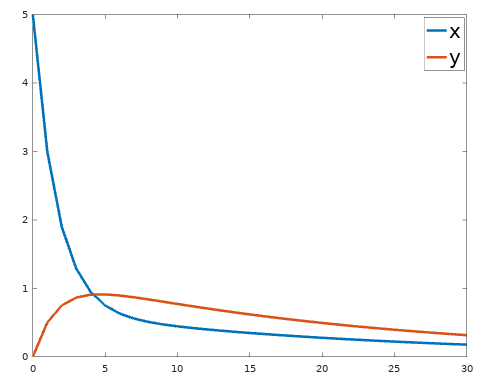
\includegraphics[width=0.6\textwidth]{coupled}\\
{\small Aside: results data was pulled from Che using SSH. Advanced students will appreciate this feature in later weeks.}
\end{center}
\end{frame}

\begin{frame}[fragile]
\frametitle{FOR Loops in C}
\begin{itemize}
\item The C FOR loop syntax is:
\begin{lstlisting}[style=CStyle]
for( initial ; condition ; increment ) {
	// Loop block
}
\end{lstlisting}
\item Where:
	\begin{itemize}
		\item \texttt{initial} is a statement executed \textit{once}
		\item \texttt{condition} is a statement executed and tested \textit{before} every loop iteration
		\item \texttt{increment} is a statement executed \textit{after} every loop iteration, but \textit{before} the \texttt{condition} is tested
	\end{itemize}
\end{itemize}
\end{frame}

\begin{frame}[fragile]
\frametitle{FOR Loops in C}
\begin{lstlisting}[style=CStyle]
for( x = 0 ; x < 10 ; x++ ) {
	printf("%d\n", x);
}
\end{lstlisting}
\begin{itemize}
\item Run this code
\item Observe that:
	\begin{itemize}
		\item 0 is printed
		\item 10 is \textbf{not} printed
		\item \texttt{x} increments automatically
	\end{itemize}

\end{itemize}
\end{frame}


\begin{frame}[fragile]
\frametitle{FOR Example 1 - Factorials}
\begin{itemize}
\item Use FOR to count from 2 to our input number
\item Keep a running product as we go
\begin{lstlisting}[style=pseudo]
BEGIN
	INPUT x
	result = 1
	FOR k = 2 TO x
		result = result * k
	ENDFOR
END
\end{lstlisting}
\item Is this algorithm robust? What happens if:
	\begin{itemize}
		\item x = -1
		\item x = 1
		\item x = 0 (\textbf{NB:} 0! = 1 because \textit{maths})
	\end{itemize}
\end{itemize}
\end{frame}

\begin{frame}
\frametitle{BREAK Statements}
\begin{itemize}
\item Sometimes you want to exit a loop \textit{before} the condition is re-tested
\item The flow-control mechanism for this is a BREAK statement
\item If executed, the loop quits
\item BREAKs typically go inside an IF
\item It adds an extra condition on loop exit placed at any point in the loop
\end{itemize}
\end{frame}

\begin{frame}[fragile]
\frametitle{FOR Example 2}
\begin{itemize}
\item Two equivalent ways to implement the $\cos()$ series from before are:
\end{itemize}
{\small\textbf{NB:} $|$\texttt{tmp}$|$ means ``absolute value of tmp''.}
\begin{multicols}{2}
\begin{lstlisting}[style=pseudo,mathescape=true,basicstyle=\ttfamily\scriptsize]
BEGIN
	INPUT x
	sum = 0
	FOR k = 0 to 10
		tmp = $\frac{(-1)^k x^{2k}}{(2k)!}$
		sum = sum + tmp
		IF |tmp| < 1e-6
			BREAK
		ENDIF
	ENDWHILE 
END
\end{lstlisting}
\columnbreak
\begin{lstlisting}[style=pseudo,mathescape=true,basicstyle=\ttfamily\scriptsize]
BEGIN
	INPUT x
	tmp = 1
	k = 0
	sum = 0
	WHILE (k<10)AND(|tmp|>1e-6)
		tmp = $\frac{(-1)^k x^{2k}}{(2k)!}$
		sum = sum + tmp
		k = k + 1
	ENDWHILE 
END
\end{lstlisting}

\end{multicols}
\end{frame}



\begin{frame}[fragile]
\frametitle{FOR Loops in C (Advanced)}
\begin{itemize}
\item \texttt{for()} syntax allows multiple expressions in the \texttt{inital} / \texttt{condition} /\texttt{increment} sections
\item Separate expressions with commas
\item eg:
\begin{lstlisting}[style=CStyle]
int x, y=10;
for( x = 0 ; x < 10 ; x++, y++ ) {
	printf("x: %d y: %d\n", x, y);
}
\end{lstlisting}
\item This increments both \texttt{x} and \texttt{y} but only \texttt{x} is used in the condition
\end{itemize}
\end{frame}

\begin{frame}[fragile]
\frametitle{Loop \texttt{continue} Statements}
\begin{itemize}
	\item A \texttt{continue} causes execution to jump back to the loop start
	\item The \textit{condition} is tested before reentry	
	\item eg, run this in the Che debugger:
	\begin{lstlisting}[style=CStyle]
int x;
for(x = 0; x < 10; x++) {
	if(x%2 == 0)
		continue;
	printf("%d is odd\n");
}
\end{lstlisting}
\item {\small(Not the best example but gets the point across)}
\end{itemize}
\end{frame}

\begin{frame}
\frametitle{\texttt{break} and \texttt{continue}}
\begin{itemize}
\item Some programmers claim that \texttt{break} and \texttt{continue} are ``naughty''
\item Well, yes, but actually no
\item They can make your code needlessly complicated
\item They might make it simpler
\item It is up to you to judge
\item As engineers you shouldn't follow strict rules
\item Always try to choose the best tool for the job
\end{itemize}
\end{frame}

\begin{frame}
\frametitle{GOTO}
\begin{itemize}
\item There exists a GOTO flow control mechanism
	\begin{itemize}
		\item Sometimes also called a \textit{branch}
	\end{itemize}
\item It ``jumps'' from one line to a different line
	\begin{itemize}
		\item An ability some consider to be unnatural
	\end{itemize}
\item It exists for a purpose
\item That purpose does not (typically) exist when writing C code
	\begin{itemize}
		\item C \textit{supports} a \texttt{goto} statement
		\item It results in ``spaghetti code'' which is hard to read
		\item Don't use it in ENGG1003
	\end{itemize}
\item You \textit{must} use branch instructions in ELEC1710
\end{itemize}
\end{frame}

\begin{frame}[fragile]
\frametitle{Loose End: Increment Example}
\begin{lstlisting}[style=CStyle,caption=\texttt{increment.c}]
#include <stdio.h>
int main() {
	int x = 0;
	int y = 0;
	int z = 0;
	y = ++x + 10;
	printf("Pre-increment: %d\n", y);
	y = z++ + 10;
	printf("Post-increment: %d\n", y);
	return 0;
}
\end{lstlisting}
Pre/post-inc/decrements have many applications, more details in coming weeks.
\end{frame}

\begin{frame}
\frametitle{Binary Nomenclature}
\begin{itemize}
\item A data type's value range is a result of the underlying binary storage mechanism
\item A single binary digit is called a \textit{bit}
\item There are 8 bits in a \textit{byte}
\item In programming we use the ``power of two'' definitions of kB, MB, etc:
	\begin{itemize}
		\item 1 kilobyte is $2^{10} = 1024$ bytes
		\item 1 Megabyte is $2^{20} = 1048576$ bytes
		\item 1 Gigabyte is $2^{30} = 1073741824$ bytes
		\item (Advanced) These numbers look better in hex: \texttt{0x3FF}, \texttt{0xFFFFF}, etc.
	\end{itemize}
\end{itemize}
\end{frame}

\begin{frame}
\frametitle{Binary Nomenclature}
\begin{itemize}
\item Observe that kilobyte, Megabyte, Gigabyte, etc use scientific prefixes
\item These \textit{normally} mean a power of 10:
	\begin{itemize}
		\item kilo- = $10^3$
		\item Mega- = $10^6$
		\item Giga- = $10^9$
		\item ...etc (see the inside cover of a physics text)
	\end{itemize}
\item Computer science stole these terms and re-defined them

\end{itemize}
\end{frame}

\begin{frame}
\frametitle{Binary Nomenclature}
\begin{itemize}
\item This has made some people \textit{illogically angry}
\item Instead, we can use a more modern standard:
	\begin{itemize}
		\item $2^{10}$ bytes = 1 kibiByte (KiB)
		\item $2^{20}$ bytes = 1 Mebibyte (MiB)
		\item $2^{30}$ bytes = 1 Gibibyte (GiB)
		\item ...etc
	\end{itemize}
\item Generally speaking, KB (etc) implies:
	\begin{itemize}
		\item powers of two to \textit{engineers}
		\item powers of ten to \textit{marketing}
			\begin{itemize}
				\item The number is smaller
				\item Hard drive manufacturers, ISPs, etc like this
			\end{itemize}
	\end{itemize}
\end{itemize}
\end{frame}

\begin{frame}
\frametitle{Unambiguous Integer Data Types}
\begin{itemize}
\item Because the standard \texttt{int} and \texttt{long} data types don't have fixed size unambiguous types exist
\item Under OnlineGDB (ie: Linux with \texttt{gcc}) these are defined in \texttt{stdint.h} (\texttt{\#include} it)
\item You will see them used commonly in embedded systems programming (eg: Arduino code)
\item The types are:
	\begin{itemize}
		\item \texttt{int8\_t}
		\item \texttt{uint8\_t}
		\item \texttt{int16\_t}
		\item ...etc
	\end{itemize}
\end{itemize}
\end{frame}

\begin{frame}[fragile]
\frametitle{Code Blocks in C}
\begin{itemize}
\item Semi-revision:
\item The curly braces \{ \} encompass a \textit{block}
\item You have used these with \texttt{if()} and \texttt{while()}
\item They define the set of lines executed inside the \texttt{if()} or \texttt{while()}

\end{itemize}
\end{frame}

\begin{frame}[fragile]
\frametitle{Code Blocks in C}
\begin{itemize}
\item You can place blocks anywhere you like
\item Nothing wrong with:
\begin{lstlisting}[style=CStyle]
int main() {
	int x;
	{
		printf("%d\n", x);
	}
	return 0;
}
\end{lstlisting}
\item This just places the \texttt{printf();} inside a block
\item It doesn't do anything useful, but...
\end{itemize}
\end{frame}

\begin{frame}[fragile]
\frametitle{Variable Scope}
\begin{itemize}
\item A variable's ``existence'' is limited to the block where it is declared
	\begin{itemize}
		\item Plus any blocks within that one
	\end{itemize}
\item Example this code won't compile:
\begin{lstlisting}[style=CStyle]
#include <stdio.h>
int main() {
	int x = 2;
	if(x == 2) {
		int k;
		k = 2*x;
	}
	printf("%d\n", k);
	return 0;
}
\end{lstlisting}
\end{itemize}
\end{frame}

\begin{frame}
\frametitle{Variable Scope}
\begin{itemize}
\item Note that \texttt{k} was declared inside the \texttt{if()}
\item That means that it no longer exists when the \texttt{if()} has finished
\item This generates a compiler error
\item It frees up some RAM
\item It also lets the variable's name be reused elsewhere
	\begin{itemize}
		\item This can be \textit{really} confusing. Be careful.
	\end{itemize}
\end{itemize}
\end{frame}


\end{document}
